\chapter{Modeling}
\section{Outline}
In this chapter \dots
\section{Ordinary Differential Equation modeling nonlinear continuous state and continuous time systems}
\subsection{Nonlinear continuous state system}
We are provided by a nonlinear continuous state system defined an ordinary differential equation which models our nonlinear system:
\[
\dot{x}(t)=f(x(t))
\]
where $X=\Re^n$ is the state space and \emph{f} is a nonlinear function defined by the vector field:
\[
f\colon\Re^n\to\Re^n
\]
In some sense the function \emph{f} assigns a "velocity" vector to each state x.
In order to find the solution of the ODE we have to assign a admissible set of initial condition and define an execution. Mathematically:
Given an initial set of states $Init \subset X$,

An execution over the time interval $\left[0,T\right)$ is a function $x\colon\left[ 0,T\right)\to \Re^n$ such that:
\begin{itemize}
	\item $x(o)\in Init$
	\item x is continuous and piece wise differentiable
	\item $x(t)=x(0)+ \int_0^t f(x(\tau))\,d\tau , \forall t \in \left[0,T\right)$
\end{itemize}

If x is a solution $\frac{dx(t)}{dt}=f(x(t)) \forall t$ for which x is differentiable.

Before looking for a solution we have to identify if a solution exists, and if does if exists locally (a solution exist over $\left[0,\delta\right)$) or globally (a solution exist over $\left[0,\infty\right)$). And also if this solution is unique (\emph{uniqueness}).

\subsection{Existence} 
\begin{thm}[Local existence]
	
	If $ f\colon\Re^n\to\Re^n$ is \emph{continuous}, then $\forall x_0$ there exist at least a solution with $x(0)=x_0$ defined on some $\left[0,\delta\right)$.
\end{thm}
\paragraph{Example} If we consider the \emph{sign function} we see that there is not a solution when the initial condition is initialized in 0: $x(0)=0$ because on any interval $\left[0,\delta\right)$ x cannot: remain zero, become positive, or become negsative.

\begin{center}
	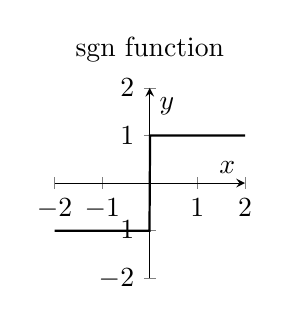
\begin{tikzpicture} 
		\begin{axis} [axis lines=middle, 
			xlabel=$x$,
			ylabel=$y$, 
			xmin=-2,xmax=2,
			ymin=-2, ymax=2,
			%grid=major,
			width=4cm, height=4cm,
			title={sgn function},
			%domain=0:150,
			samples=800] 
			\addplot [thick] {sign x}; 
			%\legend{$Legenda$};
		\end{axis} 
	\end{tikzpicture}
\end{center}

\subsection{Uniqueness}
In order to explain the uniqueness property we look at the following example:
\paragraph{Example} Consider the following ODE: 
\[
\dot{x}(t)=x(t)^{1/3}, x(0)=0.
\]
The solution of this system can be computed and it is not unique, in fact:
\begin{itemize}
	\item $x(t)=0$,
	\item $x(t)=\frac{2}{3}t^{3/2}.$
\end{itemize}
are the two solution of the system.


%% controllare la funzione non è simmetrico il disegno
\begin{center}
	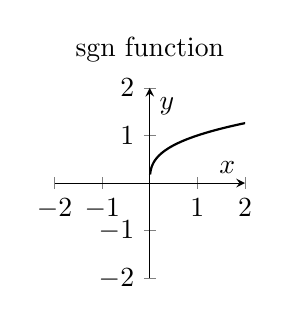
\begin{tikzpicture} 
		\begin{axis} [axis lines=middle, 
			xlabel=$x$,
			ylabel=$y$, 
			xmin=-2,xmax=2,
			ymin=-2, ymax=2,
			%grid=major,
			width=4cm, height=4cm,
			title={sgn function},
			%domain=0:150,
			samples=800] 
			\addplot [thick] {x^(1/3)}; 
			%\legend{$Legenda$};
		\end{axis} 
	\end{tikzpicture}
\end{center}

We have noticed that continuity is not enough for uniqueness, for this reason we have to make a definition:

\begin{defn} [Lipschitz conitinuity]
	$f\colon\Re^n\to\Re^n$ is \emph{Lipschitz continuous}, if in any bounded set A of $\Re^n$ there exist a constant L such that
	\[
	\|f(x_1)-f(x_2)\| \le L \|x1-x_2\|, \forall x_1,x_2 \in A.
	\]
\end{defn}

Given the definition of \emph{Lipschitz continuity} we can state the following theorem:

\begin{thm}[Local existence and uniqueness]
	If $f\colon\Re^n\to\Re^n$ is \emph{Lipschitz continuous}, then $\forall x_0$ there exist a single solution with $x(0)=x_0$ deifned on some $ \left[0,T\right)$.
\end{thm}
But since we are interested in all the time horizon we want to define \emph{global} uniqueness:
\begin{defn} [Lipschitz conitinuity]
	$f\colon\Re^n\to\Re^n$ is \emph{Lipschitz continuous}, if there exist a constant L such that
	\[
	\|f(x_1)-f(x_2)\| \le L \|x1-x_2\|, \forall x_1,x_2 \in \Re^n.
	\]
\end{defn}

Given the definition of \emph{Lipschitz continuity} we can state the following theorem:

\begin{thm}[Local existence and uniqueness]
	If $f\colon\Re^n\to\Re^n$ is \emph{Lipschitz continuous}, then $\forall x_0$ there exist a single solution with $x(0)=x_0$ deifned on $ \left[0,\infty\right)$.
\end{thm}
\paragraph{Example}
Consider the following ODE: 
\[
\dot{x}(t)=-x(t)^2, x(0)=-1.
\]
the solution is $x(t)=\frac{1}{t-1}$ but it is a local solution in $\left[0,1\right)$ since tends to $-\infty$ as $t\to 1$.
\section{Hybrid automaton modelling a hybrid system}
We will introduce this section with an example for describing the main elements of a hybrid automata.
\paragraph{Example} The thermostat
The temperature in a room is controlled by a thermostat which switch a heater on and off.
The dynamics of the temperature x (in $\SI{}{\celsius}$):
\begin{center}
	\begin{itemize}
		
		\item[heater on:] $\dot{x} = -0.2x+6 $ for $(x\to30)$
		\item[heater off:]$\dot{x}= -0.2x $  for $ (x\to 0)$
	\end{itemize} 
\end{center}

\begin{figure}[h]
	\centering
	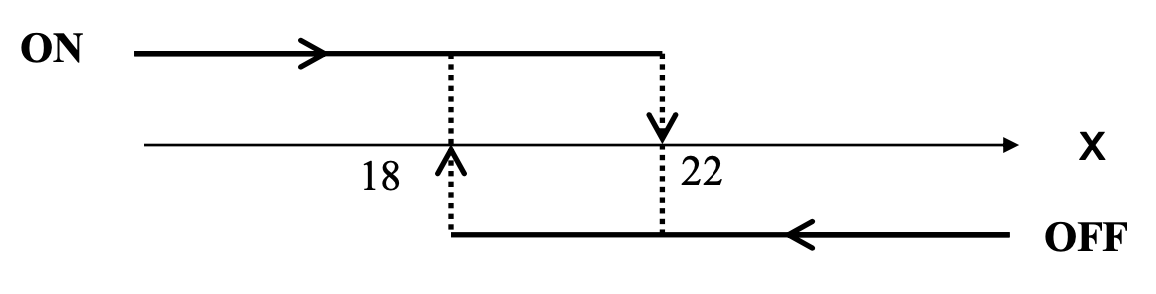
\includegraphics[scale=0.3]{immagini/hyst}
	\caption{Hysteretic Behavior}
	\label{fig:hyst}
\end{figure}

The \emph{goal} is to regulate the temperature around $\SI{20}{\celsius}$. The \emph{strategy} is to turn from OFF to ON the heater as soon as $x\le \SI{18}{\celsius}$ and turn from ON to OFF as soon as $x\ge\SI{22}{\celsius}$.

We have defined to kind of dynamics: the first one of the temperature which is \emph{continuous} and the second one of the heater strategy which is \emph{discrete}. For a better definition of the entire system we can define a \emph{hybrid dynamics} which describe the interleaved continuous and discrete dynamics.

\begin{figure}[h]
	\centering
	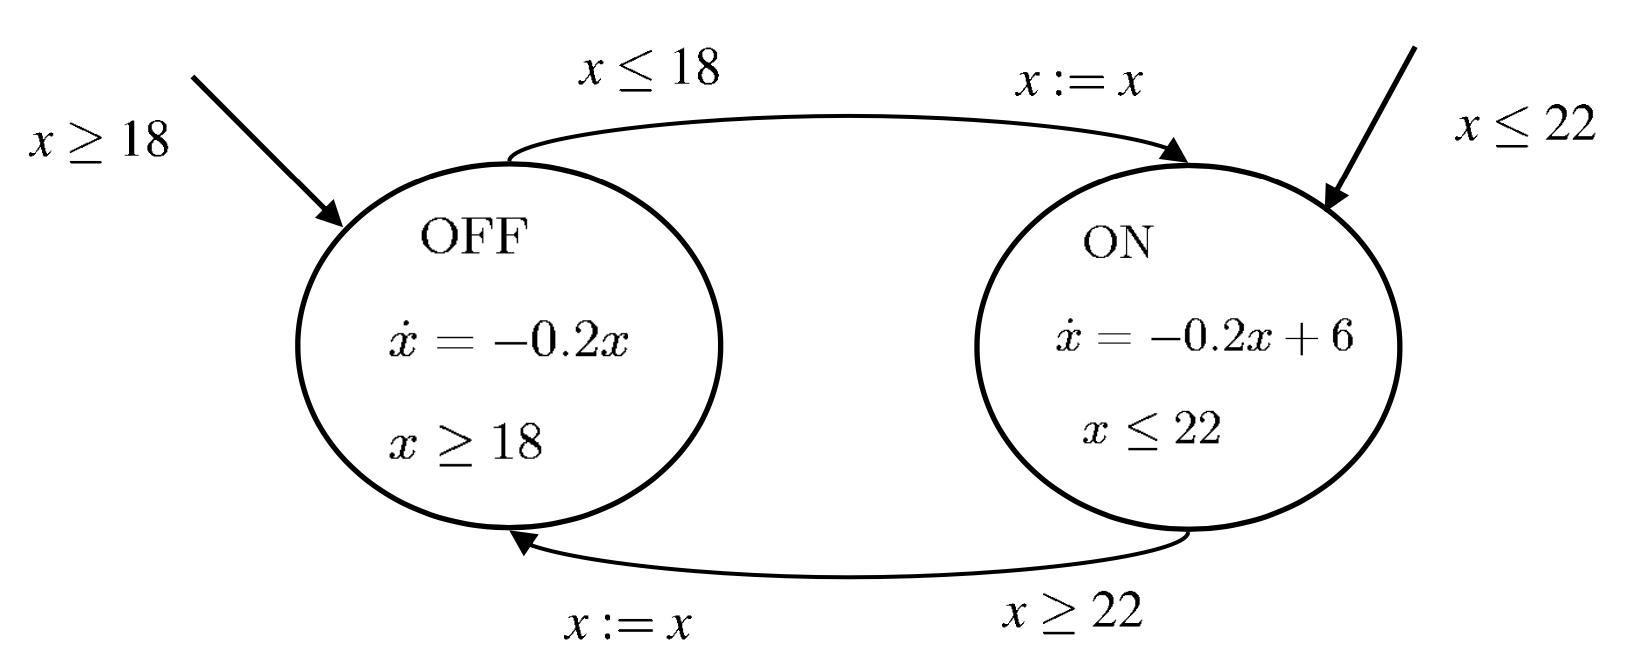
\includegraphics[scale=0.4]{immagini/thermostat}
	\caption{Hybrid dynamics}
	\label{fig:thermostat}
\end{figure}

From the graph we can conclude that e.g in the state ON an evolution can occur untill the temperature reach the boundary of the domain ($x\le22$) and then the guard conditions, if they are respected enable the deterministic transition from ON to OFF.

\subsection{Hybrid Automaton}
A hybrid automaton is a mathematical model for a dynamical system whose state $s =(q,x)$ consists of two components:
\begin{itemize}
	\item continuous state x taking values in $X\in\Re^N$;
	\item discrete state (mode) q taking values in $Q = \left\{q_1,q_2, \dots,q_N\right\}$.
\end{itemize}
Meanwhile an hybrid state space is defined as:
\[
S=Q\times X 
\]
for each value of q, the admissible values for x are only a subset of X.
For example \textcolor{red}{Dom}(q) = \textcolor{red}{domain} for x within the mode q.

The dynamics of q and x are correlated:
\begin{itemize}
	\item x follows an ODE within \textcolor{red}{Dom}(q). The ODE depends on the value of mode q;
	\item q follows a finite automaton with transition triggered by events given by x entering subsets of X called \textcolor{green}{Guards}\\
	\textcolor{green}{$\to G(q,q')$} = values for x enabling the transition from q to q';
	\item when a transition form q to q' takes place, x is reset within Dom(q') by some \textcolor{cyan}{Reset} map\\
	$\to\textcolor{cyan}{R((q,q'),x}$ = reset values for $x^+$ when a transition from q to q' occurs at x.
\end{itemize}
\begin{figure}[th]
	\centering
	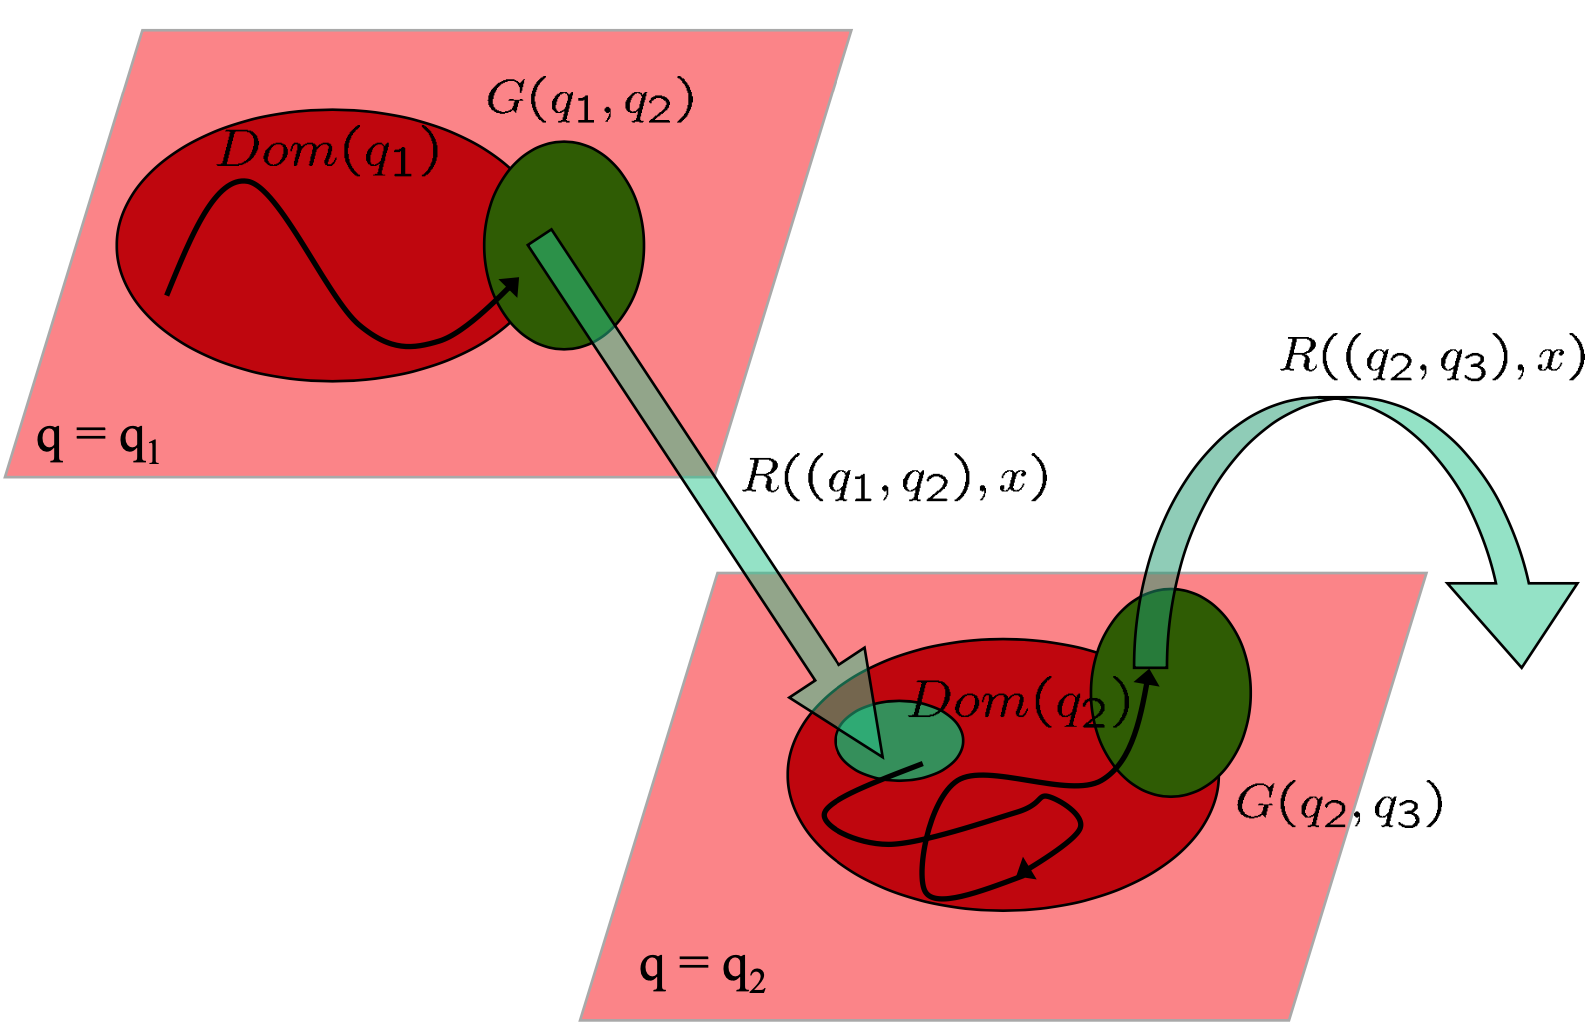
\includegraphics[scale=0.5]{immagini/trans}
	\caption{Combination of continuous evolution (black) and discrete transition (green)}
	\label{fig:trans}
\end{figure}
\subsubsection{Formal definition}
A \textcolor{red}{hybrid automaton} H is a collection H=(Q,X,f\textit{Init},Dom,E,G,R)
\begin{itemize}
	\item $Q = \left\{q_1,q_2, \dots,q_N\right\}$ is a \textcolor{green}{set of discrete states} (modes)
	\item $X=\Re^n$ is the \textcolor{green}{continuous state space}
	\item $f\colon Q\times X\to\Re^n$ is a \textcolor{green}{set of vector fields} on X
	\begin{itemize}
		\item[-] for each $q\in Q,f(q,\cdot)$ is the vector field of the ODE governing the evolution of x
		\item[-] for each $q\in Q,f(q,\cdot)$ is assumed to be \textcolor{red}{globally Lipschitz continuous}
	\end{itemize}
	\item $\emph{Init} \subseteq Q \times X$ is a \textcolor{green}{set of initial states}
	\item $Dom \colon Q \to 2^X$ assigns to each $q\in Q$ a \textcolor{green}{domain} Dom(q) of X
	\item $E \subseteq Q \times Q$ is a \textcolor{green}{set of transitions} (edges)
	\item $G\colon E\to 2^X$ is a \textcolor{green}{set of guards} (guard condition)
	\begin{itemize}
		\item[-] for each e=(q,q'), whenever x reaches G(e) from within Dom(q), transition e is enabled
	\end{itemize}
	\item $R\colon E\times X \to 2^X$ is a \textcolor{green}{set of reset maps}
	\begin{itemize}
		\item[-] for each $e=(q,q') \in E$ and $x \in Dom(q), R(e,x)\subseteq Dom(q')$ is the set of values that x can be reset to after the transition e.
	\end{itemize}
\end{itemize}
\begin{figure}[h]
	\centering
	\includegraphics[scale=0.4]{immagini/scheme}
	\caption{Graphical representation of finite automaton}
	\label{fig:scheme}
\end{figure}

\paragraph{Example}
Coming back to the previous example of the thermostat, referring to Figure \ref{fig:thermostat}, we define mathematically the components H=(Q,X,f\textit{Init},Dom,E,G,R)
\begin{itemize}
	\item $Q=\left\{ON,OFF\right\}$;
	\item $X=\Re$;
	\item $f(OFF,x)=-0.2x$; 
	\item $f(ON,x)=-0.2x+6$;
	\item $\emph{Init}=\left\{(OFF,x)\colon x\ge18\right\} \cup \left\{(ON,x)\colon x\le22\right\}$ 
	\item $Dom(OFF)=\left[18,\infty \right)$
	\item $Dom(ON)=\left(-\infty,22\right]$
	\item $E=\left\{(OFF,ON),(ON,OFF)\right\}$
	\item$G((OFF,ON))=\left(-\infty,18\right]$
	\item$G((OFF,ON))=\left[22,\infty\right)$
	\item$R(e,x)=\left\{x \right\} \forall e \in E$
\end{itemize}
\subsubsection{Execution}
To define an execution of a hybrid system, we need to introduce first the notion of
\begin{itemize}
	\item hybrid time set
	\item hybrid trajectory (which includes hybrid time set among its components)
\end{itemize}

An execution of a hybrid automaton H is a hybrid trajectory that is ''consistent'' with the definition of H.

\paragraph{Hybrid time set} A \textcolor{red}{hybrid time set} is a finite or infinite sequence of intervals $\tau = \left\{I_k,k=0,1\dots,M\right\}$ such that
\begin{itemize}		
	\item$\left[\tau_k,\tau_k'\right] $ for $ k < M$ where $\tau_k$ represent times of discrete transition
	\item$\left[\tau_M,\tau_M'\right]$ or $I_M=\left[\tau_M,\tau_M'\right) $ if $ M<\infty$;
	\item $\tau_k' = \tau_{k+1}$ that means there are no gasp and the intervals are consecutive;
	\item $\tau_k \le \tau_k'$ so intervals can be degenerated to represent multiple transitions at the same time.
\end{itemize}
\begin{figure}[h]
	\centering
	\label{fig:timeset}
	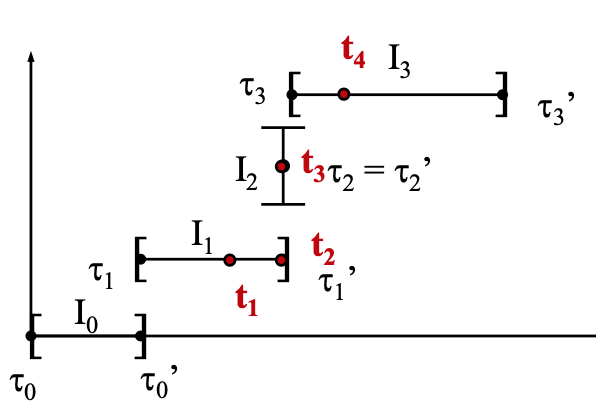
\includegraphics[scale=0.6]{immagini/time_set}
	\caption{Hybrid time set: the elements of $\tau$ are linearly ordered.}
\end{figure}

There are \textcolor{red}{two notion of length} for a hybrid time set $\tau = \left\{I_k, k=0,1,\dots,M\right\}$:
\begin{itemize}
	\item Discrete extent:
	\[<\tau>=M+1 \] that represent \textcolor{red}{number of discrete transition}
	\item Continuous extent:
	\[ \|\tau\|=\sum\limits_{k=1}^M |\tau_k'-\tau_k| \] that represent \textcolor{red}{total duration of intervals in $\tau$}
\end{itemize}
\paragraph{Classification}  Linked to the definition of \emph{length} we can differentiate three different type of time set $\tau = \left\{I_k, k=0,1,\dots,M\right\}$:
\begin{itemize}
	\item Finite: if $<\tau>$ is finite and $I_M=\left[ \tau_M,\tau_M'\right]$;
	\item Infinite: if  $<\tau>$ is infinite or $\|\tau\|$ is infinite;
	\item Zeno: if  $<\tau>$ is infinite but $\|\tau\|$ is finite.
\end{itemize}
\begin{figure}[h]
	\centering
	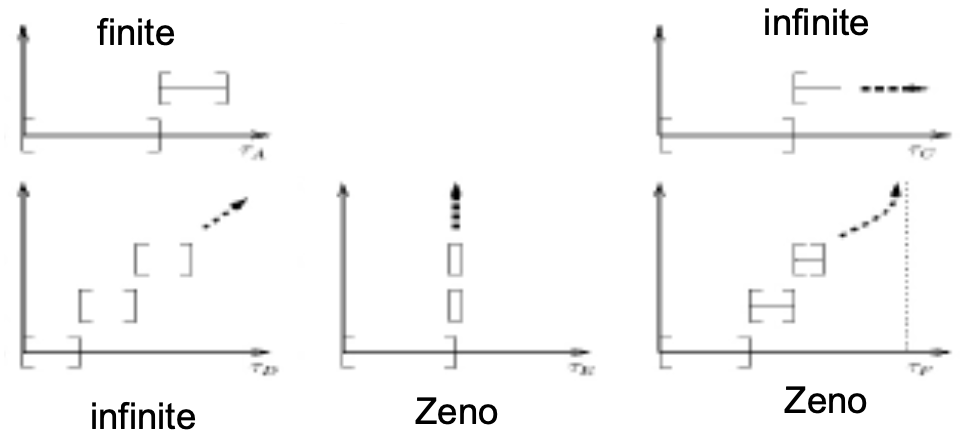
\includegraphics[scale=0.5]{immagini/classification}
	\label{fig:classification}
	\caption{Classification of the time set}
\end{figure}
To complete the fundamentals for defining an \emph{execution} of a hybrid data set we need to treat the hybrid trajectory.
\paragraph{Hybrid trajectory}
A \textcolor{red}{hybrid trajectory} is a triple ($\tau$,q,x) that consist of:
\begin{itemize}
	\item A hybrid time set $\tau = \left\{I_k, k=0,1,\dots,M\right\}$;
	\item Two sequences of functions $q = \left\{q_k(\cdot), k=0,1,\dots,M\right\}$  and $x = \left\{x_k(\cdot, k=0,1,\dots,M\right\}$ such that:
	\begin{itemize}
		\item $q_k\colon I_k\to Q$
		\item $x_k\colon I_k \to X$
	\end{itemize}
\end{itemize}
\begin{remark}
	\begin{enumerate}
		\item this is a mixture of the two notions of continuous and discrete evolution
		\item signals x and q can take multiple values at the same time instant
	\end{enumerate}
\end{remark}

Finally, since we know the concept of hybrid time set and trajectory,  we can define properly an execution:
\begin{defn} 
	A hybrid trajectory ($\tau$,q,x) is an \textcolor{red}{execution (solution) of the hybrid automaton} H=(Q,X,f\textit{Init},Dom,E,G,R) if it satisfies the following conditions:
	\begin{enumerate}
		\item \textcolor{green}{Initial condition:} $(q_0(\tau_0),x_0(\tau_0)\in \emph{Init}$
		\item \textcolor{green}{Continuous evolution:} for all j such taht $\tau_k < \tau_k'$ 
		\begin{itemize}
			\item $q_k\colon I_k\to Q$ is constant
			\item $x_k\colon I_k \to X$ is the solution of the ODE associated with $q_k(\tau_k)$
			\item $x_k(t)\in Dom(q_k(\tau_k)),t\in \left[\tau_k,\tau_k'\right)$
		\end{itemize}
		\item \textcolor{green}{Continuous evolution:} for all j such that $\tau_k < \tau_k'$ 
		\begin{itemize}
			\item $q_k(\tau_k'),q_{k+1}(\tau_{k+1})\in E$ transition is feasible
			\item $x_k(\tau_k')\in G(q_k(\tau_k'),q_{k+1}(\tau_{k+1}$ guard condition satisfied
			\item $x_{k+1}(\tau_{k+1})\in R((q_{k+1}(\tau_{k+1})),x_k(\tau_k')$ reset condition satisfied
		\end{itemize}
	\end{enumerate}
\end{defn}
So now we want analyze that situation in which the execution can go wrong. From the side of problems concerning the ODE solution (like existence, uniqueness, finite escape) we know we are fine thanks to the assumption of Lipschitz global continuity. But problems can arise also due the hybrid nature of the system. The problem we want to analyze are:
\begin{itemize}
	\item Zeno;
	\item chattering;
	\item blocking;
	\item nondeterministic.
\end{itemize}

\subsubsection{Problem and solution of the hybrid execution }
\paragraph{Zeno} Let ($\tau$,q,x) be an execution of H. ($\tau$,q,x)  is called \textcolor{red}{Zeno execution} if $\tau = \left\{I_k, k=0,1,\dots,M\right\}$ is Zeno (infinite number of discrete transition in finite time)\\
\paragraph{Chattering} Let ($\tau$,q,x) be an execution of H. ($\tau$,q,x)  is called \textcolor{red}{chattering execution} if $\tau = \left\{I_k, k=0,1,\dots,M\right\}$ is Zeno (infinte number of discrete transition in finite time and after some $h \ge 0$, all the intervals $I_k,k \ge h$, are singletons.\\
In practice this means that after a certain time instant the continuous transition remains constant while the discrete transitions occurs infinite times in a finite time set.\\
A possible solution of this problem is called \textbf{temporal regularization} and consist to add a sort of delay between two discrete transition such that we avoid infinite number of discrete transition in finite time. 
\paragraph{Example}[The Bouncing Ball]
We want to analyze the situation of a ball bouncing along vertical axis freely. We can identify two situations: ball flying in the air and ball hitting the ground. The state of the system are the position $x_1$ and the velocity $x_2$. In Figure
\begin{figure}[h]
	\centering
	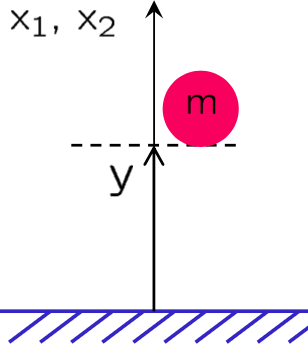
\includegraphics[scale=0.4]{immagini/bouncing ball}
	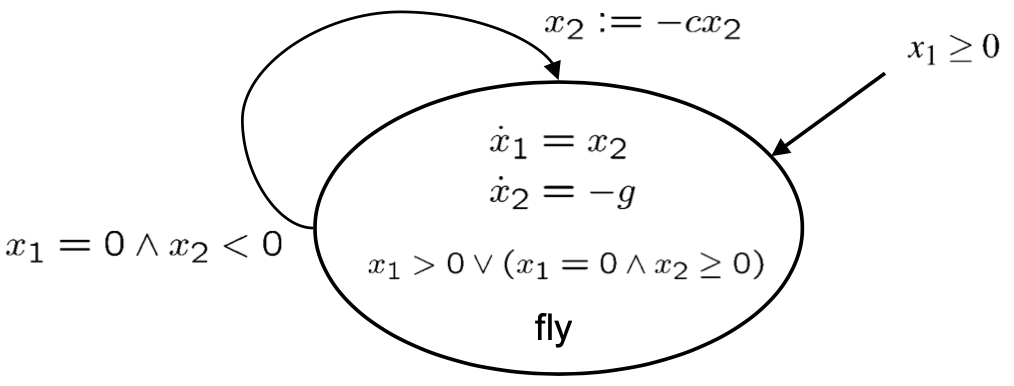
\includegraphics[scale=0.4]{immagini/bb_automata}
	\caption{Bouncing ball model}
	\label{fig:bbautomata}
\end{figure}
The mathematical description of the components H=(Q,X,f\textit{Init},Dom,E,G,R) is:
\begin{itemize}
	\item $Q=\left\{fly\right\}$;
	\item $X=\Re^2$;
	\item $f(fly,x)=[x_2,-g]^T$; 
	\item $\emph{Init}=\left\{(fly,(x_1,x_2))\colon x_1\ge0\right\}$ 
	\item $Dom(fly)=\left\{(x_1,x_2)\colon x_1>0\right\} \cup \left\{(x_1,x_2)\colon x_1= 0, x_2\ge 0 \right\}$;
	\item $E=\left\{(fly,fly)\right\}$
	\item$G((fly,fly))=\left\{(x_1,x_2)\colon x_1= 0, x_2<0 \right\}$
	\item$R(e,(x_1,x_2))=\left\{(x_1,-cx_2) \right\} \forall e \in E$
\end{itemize}
Since for $x_1(0)=0, x_2(0)>0$ occurs infinite number of transitions in finite time this is a \textcolor{red}{Zeno} hybrid system.
Implementing the possible solution we have described before we obtain the following diagram associated to the following evolution of the states.
\begin{figure}[h]
	\centering
	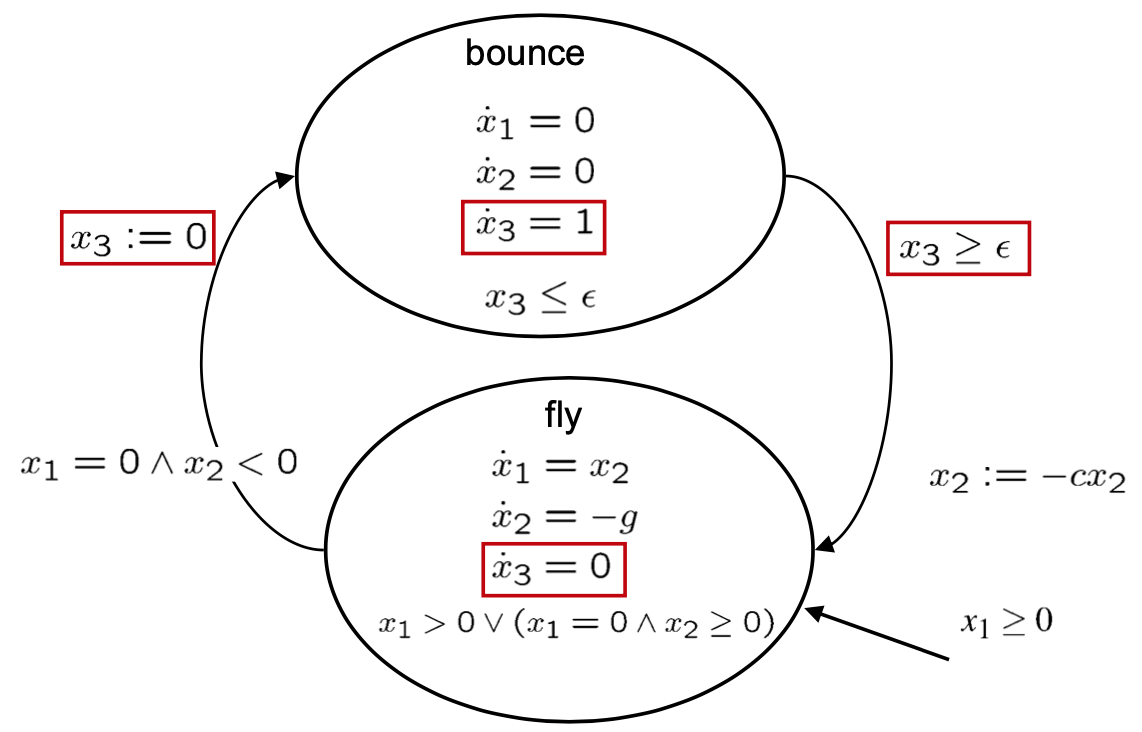
\includegraphics[scale=0.3]{immagini/corrected_bb_automata}
	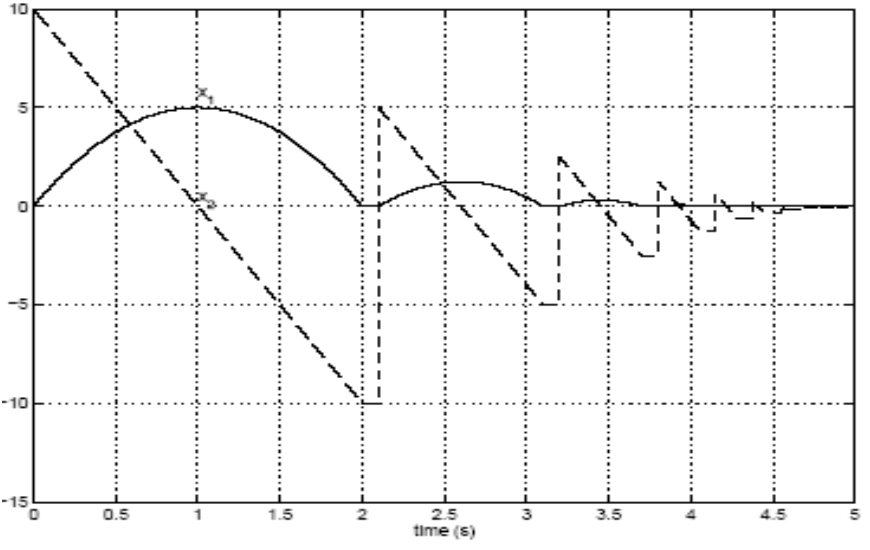
\includegraphics[scale=0.3]{immagini/evolution_bb}
	\caption{Correction of Zeno system with temporal delay equal to 0.1}
	\label{fig:bbautomata_corrected}
\end{figure}
Let's now treat the last two problems: the blocking system and the nondeterministic.
\subsubsection{Blocking vs Non-Blocking}
A \textcolor{red}{hybrid automaton} H=(Q,X,f\textit{Init},Dom,E,G,) is \textcolor{red}{non-blocking} if for all initial states $(q,x) \in \emph(Init)$ there is an infinite execution starting at (q,x).
\begin{remark}
In practice this is only a \textbf{sufficient condition} because there can be a condition that if it is reached the system blocks but it is not mandatory that this condition is reached.
\end{remark}
Let's give now a formal definition of this concept.
\begin{defn}
	Given a hybrid automaton  H=(Q,X,f\textit{Init},Dom,E,G,R), \textcolor{red}{transition states} are those states from which continuous evolution is impossible:
	\[
	Trans:=\left\{(q',x')\in Q\times X\colon \forall \delta>0,\exists t \in[0,\delta] \text{such that} \, x(t)\notin Dom(q')\right\}
	\] where x(t) is the solution of $\frac{dx}{dt}=f(q',x) \text{with} \, x(0)=x'$.
\end{defn}
\begin{tcolorbox}
	A hybrid automaton is non-blocking if:
	\begin{enumerate}
		\item $f(q,\cdot)$ is globally Lipschitz for each $q\in Q$;
		\item for eah $(q,x)\in Trans$, there exists q' such that $(q,q')\in E$ and $x \in G(q,q')$ 
	\end{enumerate}
\end{tcolorbox}
\paragraph{Example}
Let's look at the automata in Figure \ref{fig:non-blocking}:
considering the following state$\left\{(q_2,x)\colon x\le 0\right\} \subseteq Trans$ we notice that is trivial fo $x<0$ because the continuous state is outside $Dom(q_2)$, so for $x=0$ it would exit domain. Even if  there are no discrete transition possible from $q_2$ it is still non blocking because for all initial states $(q,x)\in Init$ there is an infinite execution starting at (q,x).
\begin{figure}[h]
	\centering
	\includegraphics[scale=0.4]{"immagini/non blocking"}
	\caption{Non blocking hybrid automata}
	\label{fig:non-blocking}
\end{figure}
\subsubsection{Deterministic vs Nondeterministic}
\begin{defn}{Maximal execution}
	An execution is maximal if \emph{it cannot be extended any further}.
\end{defn}
A \textcolor{red}{hybrid automaton} H=(Q,X,f\textit{Init},Dom,E,G,) is \textcolor{red}{deterministic} if for all initial states $(q,x) \in \emph(Init)$ there exists \textcolor{red}{at most one maximal execution} starting at (q,x).\\
But concretely what does cause non determinism?

\begin{SCfigure}[][h]
	\centering
	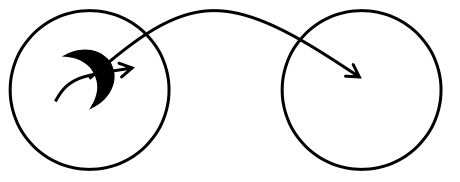
\includegraphics[scale=0.35]{immagini/nd_1}
	\caption{choice between continuous evolution and discrete transitions}
	\label{fig:nd_1}
\end{SCfigure}
\begin{SCfigure}[][h]	
	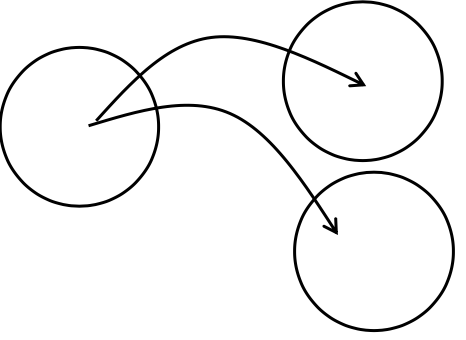
\includegraphics[scale=0.35]{immagini/nd_2}
	\caption{Discrete transitions to multiple modes are jointly enabled}
	\label{fig:nd_2}
\end{SCfigure}
\begin{SCfigure}[][!h]	
	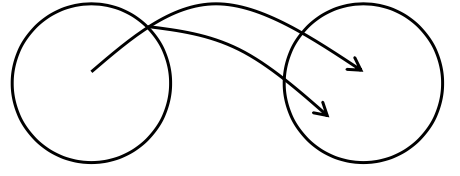
\includegraphics[scale=0.35]{immagini/nd_3}
	\caption{multiple reset positions}
	\label{fig:nd_3}
\end{SCfigure}
 Finally we can summarize the definition if \emph{deterministic} as follow: 
\begin{tcolorbox}
	A hybrid automaton is non-blocking if:
	\begin{enumerate}
		\item a discrete transitions occur only when continuous evolution is not possible;
		\item o multiple discrete transitions are possible at the same time;
		\item there is only one reset position when taking a discrete transition.
	\end{enumerate}
\end{tcolorbox}
\subsubsection{Existence and uniqueness if executions}
A hybrid automaton has a \textcolor{red}{unique infinite execution for each initial state if it is non-blocking and deterministic}.\\
\\
This is a sufficient condition given by  putting together the \textcolor{red}{sufficient conditions for the hybrid automaton to be non- blocking and deterministic}.\\
Formally speaking the conclusion of this section can be summarized like that:
\begin{tcolorbox}
	A hybrid automaton has a \textcolor{red}{unique infinite execution} for each initial state if
	\begin{enumerate}
		\item $f(q,\cdot)$ is globally Lipschitz for each $q\in Q$;
		\item for eah $(q,x)\in Trans$, there exists q' such that $(q,q')\in E$ and $x \in G(q,q')$ \\ \emph{(a discrete transition should be possible from the Trans states)
		}
		\item If $x \in G(q,q')$ for some $(q,q') in E$, then $(q,x) \in Trans$\\ \emph{(discrete transitions occur only when continuous evolution is not possible)}
		\item If $(q,q'),(q,q'')\in E$, then $G(q,q')\cap G(q,q'')=\emptyset$ \\ \emph{(no multiple discrete transitions are possible at the same time)}
		\item If $(q,q')\in E$ and $x\in G(q,q')$, then $R((q,q'),x)$ is a singleton\\ \emph{(only one reset position when taking a discrete transition)}
	\end{enumerate}
\end{tcolorbox}

%%%% Fine capitolo 1%%%%%